\documentclass{article}[12pt]
\linespread{1.5}

%sets page formatting
\setlength{\textheight}{9truein}
\setlength{\topmargin}{-0.9truein}
\setlength{\parindent}{0pt}
\setlength{\parskip}{10pt}
\setlength{\columnsep}{.4in}
\counterwithin*{equation}{section}
\counterwithin*{equation}{subsection}

%macros for shortened typing
\newcommand{\beq}{\begin{equation}}
\newcommand{\eeq}{\end{equation}}

\usepackage{enumerate}
\usepackage{pgfplots}
\usepackage{float}
\usepackage{tikz}
\usepackage{tcolorbox}
\usepackage{amsmath}
\usepackage{amssymb}
\usepackage{caption}
\usetikzlibrary{angles, quotes}
\usepackage[margin=0.5in,top=1.0in,bottom=1.0in]{geometry}



\begin{document}
\begin{titlepage}
   \begin{center}
       \vspace*{1cm}
 
       \textbf{Uniform Circular Motion Lab}
 
       \vspace{0.5cm}
 
       \vspace{1.5cm}
 
       \textbf{Nithin Muthukumar, Judy Dong, Anamta Masoodi, Zihan Dong}
 
       \vspace{0.8cm}
 
       SPH4UN-01
       \vspace{0.2cm}
       
       November 16 2019
 
   \end{center}
\end{titlepage}

\pagestyle{plain}
\section*{Question}
What is the relationship between the frequency of revolution and:
\begin{enumerate}[i.]
\item The magnitude of the {\bf force} causing the circular motion?
\item The {\bf radius} of the circular path?
\item The {\bf mass} of the object?
\end{enumerate}

\section*{Hypothesis}
\begin{enumerate}[i.]
\item 
If the magnitude of centripetal force increases, then frequency will increase as well since they are directly proportional. According to Newton's second law $F_{net}=ma$, force is directly proportional to acceleration. Also, using the kinematics formula $a=\frac{v}{t}$ it can be seen that acceleration is inversely proportional to time and by extension, force is also inversely proportional to time. Since period is the time it takes to complete a revolution and frequency is the number of cycles per second, period and frequency are inversely proportional which can also be seen from the formula $f=\frac{1}{t}$. By combining the relationship between time and force with the relationship between period and frequency it can be concluded that $f\propto F_c$.\\\\
\begin{tikzpicture}

\begin{axis}[xmax=10,xmin=0,ymax=10,ymin=0,xticklabels=\empty,yticklabels=\empty,xlabel=Centripetal Force (N),ylabel=Frequency (Hz),title=Frequency vs. Centripetal Force]
\addplot[domain=0:100] expression {x};
\end{axis}
\end{tikzpicture}\\
\item
If the radius of the circular path increases, the frequency will decrease because frequency and radius are inversely proportional. The distance travelled by an object in circular motion is the circumference which is directly proportional to the radius. Since $v=\frac{d}{t}$, distance is directly proportional to time. By the logical conclusion that distance increases as the radius increases and that it takes longer to travel a larger distance, we can see that radius is directly proportional to time. Since period is the time taken for one cycle and frequency is inversely proportional to the period, it can be concluded that $f\propto\frac{1}{r}$.\\\\
\begin{tikzpicture}
\begin{axis}[xmax=10,xmin=0,ymax=10,ymin=0,xticklabels=\empty,yticklabels=\empty,xlabel=Radius (m),ylabel=Frequency (Hz),title=Frequency vs. Radius ,samples=2000]
\addplot[domain=0:100]  expression {1/x};
\end{axis}
\end{tikzpicture}\\
\item
If the mass of the object increases, then the frequency will decrease as they are inversely proportional. The mass of an object is inversely proportional to its acceleration as shown in Newton's second law of motion. Acceleration is also inversely proportional to time which makes mass directly proportional to time. Since frequency is inversely proportional to time, $f\propto \frac{1}{m}$.\\\\
\begin{tikzpicture}
\begin{axis}[xmax=10,xmin=0,ymax=10,ymin=0,xticklabels=\empty,yticklabels=\empty,xlabel=Mass (g),ylabel=Frequency (Hz),samples=100,title=Frequency vs. Mass,samples=2000]
\addplot[domain=0:100]  expression {1/x};
\end{axis}
\end{tikzpicture}\\
\end{enumerate}
%Analysis
\section*{Analysis}
%table 1
\subsection{Experimental Data}
\begin{table}[H]
\centering
\caption{Changing Mass}
\begin{tabular}{c c c c c c}
\hline\hline
Mass (kg) &Force of Tension (N) &Trial 1 (s)&  Trial 2 (s) & Average Time (s)& frequency \\ [0.5ex] % inserts table %heading
\hline
0.100&0.981&12.77&13.44&13.11&1.53 \\
0.150&1.4715&9.89&10.38&10.14&1.97 \\
0.200&1.962&9.10&9.82 &9.46&2.11 \\
0.250 &2.4525& 8.50 & 8.22 & 8.36 & 2.39 \\
0.300 &2.943& 7.27 & 7.43 & 7.35 & 2.72 \\ [1ex]
\hline
\end{tabular}
\end{table}
\begin{tcolorbox}[title=\begin{center}Table 1: Constants\end{center}]
\centering
Number of Stoppers: 1\\
Stopper Mass: 0.021 kg\\
Radius: 0.6m
\end{tcolorbox}

\begin{table}[H]
\centering
\caption{Changing Radius}
\begin{tabular}{c c c c c}
\hline\hline
Radius (m) & Trial 1 (s)&  Trial 2 (s) & Average Time (s)& frequency \\ [0.5ex] % inserts table %heading
\hline
0.40&7.96&7.89&7.93&2.52 \\
0.50&8.92&8.84&8.88&2.25 \\
0.60&9.31&9.42&9.37&2.14 \\
0.70 &10.93 &11.05& 10.99 & 1.82 \\
0.80 &12.10&11.48& 11.79 & 1.70 \\ [1ex]
\hline
\end{tabular}
\label{table:massChange}

\end{table}
\begin{tcolorbox}[title=\begin{center}Table 2: Constants\end{center}]
\centering
Number of Stoppers: 1\\
Stopper Mass: 0.021 kg\\
Mass: 0.2 kg

\end{tcolorbox}
\begin{table}[H]
\centering
\caption{Changing Number of Stoppers}
\begin{tabular}{c c c c c c}
\hline\hline
Number Of Stoppers&Total Mass (kg)& Trial 1 (s)&  Trial 2 (s) & Average Time (s)& frequency \\ [0.5ex] 
\hline
1&0.021&9.25&8.96&9.105&2.20 \\
2&0.042&12.46&12.34&12.40&1.61 \\
3&0.063&16.00&16.60&16.30 &1.23\\
4&0.084&18.34&18.06&18.20 &1.10\\
5&0.095&18.78&18.84& 18.81 &1.06\\ [1ex]
\hline
\end{tabular}
\label{table:massChange}

\end{table}
\begin{tcolorbox}[title=\begin{center}Table 3: Constants\end{center}]
\centering
Stopper Mass: 0.021 kg\\
Radius: 0.6m\\
Mass: 0.2 kg\\
\end{tcolorbox}
\subsection*{Graphing Relations}
\subsubsection*{Frequency and Tension}
Since tension is constant along the string, the force of tension is equal to the force of gravity since $F_{net}$ is 0 because the string does not slide up or down.\\
\begin{tikzpicture}
\begin{axis}[
width=0.55\textwidth,
    title={Frequency vs. Tension},
    xlabel={Tension (N)},
    ylabel={Frequency (Hz)},
    xmin=0, xmax=5,
    ymin=0, ymax=5,
    xtick={0,0.5,1,1.5,2,2.5,3,3.5,4,4.5,5},
    ytick={0,0.5,1,1.5,2,2.5,3,3.5,4,4.5,5},
    ymajorgrids=true,
    xmajorgrids=true
]
 
\addplot[
    only marks=true,
    color=blue,
    mark=x
    ]coordinates {(0.981,1.53)(1.4715,1.97)(1.962,2.11)(2.4525,2.39)(2.943,2.72)};
\addplot[domain=0:100,samples=1000]  expression {1.2*sqrt(x)+0.5};
 
\end{axis}
\end{tikzpicture}\\
Based on the graph above, $f \not\propto F_t$ which means that the hypothesis is wrong. However, the graph is similar to $f(x)=\sqrt{x}$\\

\begin{tikzpicture}
\begin{axis}[
width=0.55\textwidth,
    title={Frequency Squared vs. Tension},
    xlabel={Tension (N)},
    ylabel={Frequency Squared ($Hz^2$)},
    xmin=0, xmax=5,
    ymin=0, ymax=10,
    xtick={0,0.5,1,1.5,2,2.5,3,3.5,4,4.5,5},
    ytick={0,1,2,3,4,5,6,7,8,9,10},
    ymajorgrids=true,
    xmajorgrids=true
]
 
\addplot[
    mark=x,
    only marks=true,
    color=blue
    ]coordinates {(0.981,2.3409)(1.4715,3.8809)(1.962,4.4521)(2.4525,5.7121)(2.943,7.3984)};
\addplot[domain=0:100,samples=1000]  expression {2.2*x+0.5};
 
\end{axis}
\end{tikzpicture}\\
Based on the graph above it is clear that $f \propto \sqrt{F_t}$

\subsubsection*{Frequency and Radius}
\begin{tikzpicture}
\begin{axis}[
width=0.55\textwidth,
    title={Frequency vs Radius},
    xlabel={Radius (m)},
    ylabel={Frequency (Hz)},
    xmin=0, xmax=1,
    ymin=0, ymax=5,
    xtick={0,0.1,0.2,0.3,0.4,0.5,0.6,0.7,0.8,0.9,1},
    ytick={0,0.5,1,1.5,2,2.5,3,3.5,4,4.5,5},
    ymajorgrids=true,
    xmajorgrids=true
]
 
\addplot[
    only marks=true,
    color=blue,
    mark=x
    ]coordinates {(0.4,2.52)(0.5,2.25)(0.6,2.14)(0.7,1.82)(0.8,1.7)};
\addplot[domain=0:1,samples=1000]  expression {1.2/sqrt(x)+0.5};
\end{axis}
\end{tikzpicture}\\
Based on the graph above, $f \not\propto r$ \\\\
\begin{tikzpicture}
\begin{axis}[
width=0.55\textwidth,
    title={Inverse of Frequency vs Radius},
    xlabel={Radius (m)},
    ylabel={Inverse of Frequency ($\frac{1}{Hz}$)},
    xmin=0, xmax=1,
    ymin=0, ymax=1,
    xtick={0,0.1,0.2,0.3,0.4,0.5,0.6,0.7,0.8,0.9,1},
    ytick={0,0.1,0.2,0.3,0.4,0.5,0.6,0.7,0.8,0.9,1},
    ymajorgrids=true,
    xmajorgrids=true
]
 
\addplot[
    only marks=true,
    color=blue,
    mark=x
    ]coordinates {(0.4,0.3968)(0.5,0.44444)(0.6,0.467289)(0.7,0.54945)(0.8,0.588235)};
\addplot[domain=0:1,samples=1000]  expression {0.606*sqrt(x)+0.025};
\end{axis}
\end{tikzpicture}\\
Based on the graph above, $f \not\propto r$ which proves that the hypothesis was wrong.\\\\

\begin{tikzpicture}
\begin{axis}[
   width=0.55\textwidth,
    title={Inverse of Frequency Squared vs Radius},
    xlabel={Radius (m)},
    ylabel={Frequency (Hz)},
    xmin=0, xmax=1,
    ymin=0, ymax=0.5,
    xtick={0,0.1,0.2,0.3,0.4,0.5,0.6,0.7,0.8,0.9,1},
    ytick={0,0.05,0.1,0.15,0.2,0.25,0.3,0.35,0.4,0.45,5},
    ymajorgrids=true,
    xmajorgrids=true
]
 
\addplot[
    only marks=true,
    color=blue,
    mark=x
    ]coordinates {(0.4,0.15745)(0.5,0.1975304681)(0.6,0.218359)(0.7,0.3018953)(0.8,0.34602)};
\addplot[domain=0:1,samples=100]  expression {0.495*x-0.05};
\end{axis}
\end{tikzpicture}\\
Based on the graph above, $f \propto \frac{1}{\sqrt{r}}$ which proves that the hypothesis was wrong.
\subsubsection*{Frequency and Mass of Object in Motion}
\begin{tikzpicture}
\begin{axis}[
    width=0.55\textwidth,
    title={Frequency vs Mass of Object},
    xlabel={Mass (kg)},
    ylabel={Frequency (Hz)},
    xmin=0, xmax=0.1,
    ymin=0, ymax=5,
    xtick={0,0.01,0.02,0.03,0.04,0.05,0.06,0.07,0.08,0.09,0.1},
    ytick={0,0.5,1,1.5,2,2.5,3,3.5,4,4.5,5},
    ticklabel style={ 
/pgf/number format/fixed, 
/pgf/number format/precision=5 
}, scaled ticks=false ,
    ymajorgrids=true,
    xmajorgrids=true
]
 
\addplot[
    only marks=true,
    color=blue,
    mark=x
    ]coordinates {(0.021,2.20)(0.042,1.61)(0.063,1.23)(0.084,1.10)(0.095,1.06)};
\addplot[domain=0:0.1,samples=100]  expression {0.438/sqrt(x+0.01)-0.32};
\end{axis}
\end{tikzpicture}\\
Based on the graph above, $f \not\propto r$ \\\\
\begin{tikzpicture}
\begin{axis}[
    width=0.55\textwidth,
    title={Inverse of Frequency vs Mass of Object},
    xlabel={Mass of Object (kg)},
    ylabel={Inverse of Frequency ($\frac{1}{Hz}$)},
    xmin=0, xmax=0.1,
    ymin=0, ymax=5,
    xtick={0,0.01,0.02,0.03,0.04,0.05,0.06,0.07,0.08,0.09,0.1},
    ytick={0,0.5,1,1.5,2,2.5,3,3.5,4,4.5,5},
    ticklabel style={ 
/pgf/number format/fixed, 
/pgf/number format/precision=5 
}, scaled ticks=false ,
    ymajorgrids=true,
    xmajorgrids=true
]
 
\addplot[
    only marks=true,
    color=blue,
    mark=x
    ]coordinates {(0.021,0.45454545)(0.042,
0.6211180124)(0.063,0.8130081301)(0.084,0.9090909091)(0.095,0.9433962264)};
\addplot[domain=0:0.1,samples=1000]  expression {2*sqrt(x)+0.27};
\end{axis}
\end{tikzpicture}\\
Based on the graph above, $f \not\propto \frac{1}{r}$ which proves that the hypothesis was wrong.\\\\

\begin{tikzpicture}
\begin{axis}[
    width=0.55\textwidth,
    title={Inverse Frequency Squared vs Mass},
    xlabel={Radius (m)},
    ylabel={Frequency (Hz)},
    xmin=0, xmax=0.1,
    ymin=0, ymax=1,
    xtick={0,0.01,0.02,0.03,0.04,0.05,0.06,0.07,0.08,0.09,0.1},
    ytick={0,0.1,0.2,0.3,0.4,0.5,0.6,0.7,0.8,0.9,1},
    ymajorgrids=true,
    xmajorgrids=true,
    ticklabel style={ 
/pgf/number format/fixed, 
/pgf/number format/precision=5 
}, scaled ticks=false ,
    ymajorgrids=true,
    xmajorgrids=true
]
]
 
\addplot[
    only marks=true,
    color=blue,
    mark=x
    ]coordinates {(0.021,0.2066115702)(0.042,0.3857875853)(0.063,0.6609822196)(0.084,0.826446281)(0.095,0.88999644)};
\addplot[domain=0:0.1,samples=1000]  expression {10*x};
\end{axis}
\end{tikzpicture}\\
Based on the graph above, $f \propto \frac{1}{\sqrt{r}}$ which proves that the hypothesis was wrong.
%all graphs done
\subsection*{Deriving the equation for frequency}
The three proportionality statements derived from the graphs are:\\

\beq f\propto\frac{1}{\sqrt{r}}\eeq\\
\beq f\propto\frac{1}{\sqrt{m}} \eeq\\
\beq f\propto\sqrt{F_c} \eeq\\
By combining the three equations it yields:\\

\begin{equation*} 
f\propto\sqrt{\frac{F_c}{mr}}
\end{equation*}\\
This means that $f$ grows at the same rate as $\sqrt{\frac{F_c}{mr}}$. \\To derive an equation a constant k is introduced.

$\therefore f=k\sqrt{\frac{F_c}{mr}}$\\\\
Where k is the constant of proportionality.

\subsection{Verifying K Values}

Using the equation above, the k values can be derived from each data point using the constants, independent variables (magnitude of centripetal force, mass of object and radius) and the frequency of the trial.

\begin{table}[H]
\centering
\caption*{K Values}
\begin{tabular}{c c c c c}

\hline\hline
Mass (kg)&Radius (m)& $F_c$ (N)&Frequency (Hz)&k \\ [0.5ex] 
\hline
0.021&0.60&0.981&1.53&0.173\\
0.021&0.60&1.47&1.97&0.182\\
0.021&0.60&1.96&2.11&0.169\\
0.021&0.60&2.45&2.39&0.171\\
0.021&0.60&2.94&2.72&0.178\\
0.021&0.40&1.96&2.52&0.165\\
0.021&0.50&1.96&2.25&0.165\\
0.021&0.60&1.96&2.14&0.172\\
0.021&0.70&1.96&1.82&0.158\\
0.021&0.80&1.96&1.70&0.157\\
0.021&0.60&1.96&2.20&0.176\\
0.042&0.60&1.96&1.61&0.182\\
0.063&0.60&1.96&1.23&0.170\\
0.084&0.60&1.96&1.10&0.176\\
0.095&0.60&1.96&1.06&0.181\\[1ex]
\hline
\end{tabular}
\label{table:massChange}
\end{table}
All k values obtained by using the above formula are within a reasonable range which indicates that the experiment was accurate and that the formula obtained through graphing is correct.\\\\
$\frac{0.173+0.182+0.169+1.171+0.178+0.165+0.172+0.158+0.157+0.176+0.182+0.170+0.176+0.181}{15}$\\
\\$= 0.172 $\\\\
$f=0.172\sqrt{\frac{F_c}{mr}}$
\subsection{Comparison With Formula For Centripetal Force}
By using the formula for centripetal force we can rearrange to obtain the formula for f. The value of the constants in this equation can be calculated to determine the actual constant of proportionality.
\begin{eqnarray*}
  F_c=\frac{mv^2}{r} \\\\
  F_c=4\pi^2mrf^2\\\\
  f=\sqrt{\frac{F_c}{4\pi^2mr}}\\\\
  f=0.159\sqrt{\frac{F_c}{mr}}\\\\
\end{eqnarray*}

\begin{eqnarray*}
\%Error=\frac{measured-accepted}{accepted}*100\%\\\\
\%Error=\frac{0.172-0.159}{0.159}*100\%\\\\
\%Error=8.18\%
\end{eqnarray*}


According to the formula for $F_c$, k should be equal to 0.159. The actual calculated k value is 0.172. The percent error of our experimental data is 8.18\% The discrepancy could have been caused by random and systematic error that occurs during trials.

\subsection{Free Body Diagram of Situation}
%fbd
For this experiment, the expected situation was a perfectly horizontal circular motion where $F_t=F_g$ due to $F_{net}$ being 0:\\
\begin{tikzpicture}
\coordinate (Origin) at (1,1);
\draw (0,0) rectangle (2,2);
\draw (1,1) -- (1,-1.5);
\draw[->] (1,1) -- (1,-1.5) node[right] {$F_g$};
\draw[->] (1,1) -- (-1,1) node[left]{$F_t$} coordinate (ft);
\draw[<-] (0,3) -- (1,3) node[above] {$F_{net}$};
\end{tikzpicture}\\
In reality, the experiment had a conical rotation because there needs to be a vertical component counteracting the $F_g$ of the mass at the end of the string to make $F_{net}$ equal to 0.\\
\begin{tikzpicture}
\coordinate (Origin) at (1,1);
\draw (0,0) rectangle (2,2);
\draw (1,1) -- (1,-1.5);
\draw[->] (1,1) -- (1,-1.5) node[right] {$F_g$};
\draw[->] (1,1) -- (-1,2) node[left]{$F_t$} coordinate (ft);
\draw[dashed] (1,1) -- (-1,1) coordinate (axis);
\draw pic["$\theta$", draw=orange, text=orange, <->, angle eccentricity=1.25, angle radius=1cm] {angle=ft--Origin--axis};
\draw[<-] (0,3) -- (1,3) node[above] {$F_{net}$};
\end{tikzpicture}

\section*{Evaluation}

{\bf F. What happens to the accuracy as the frequency of revolution of the stopper increases?}\\ As the frequency of revolution of the stopper increases (with other variables held constant), the accuracy increases as the angle that the string makes with the horizontal decreases as frequency increases. This can be proved using the equation $F_tcos\theta = 4\pi^2mrf^2$, which shows that $f \propto cos\theta$. As the frequency increases, the value of cos$\theta$ increases. A smaller value angle will yield a larger value of cos$\theta$, so as cos$\theta$ increases, the angle that the string makes with the horizontal decreases, causing the tension force acting on the stopper to be closer to the horizontal, so the value of $F_t$ will approach $F_c$, thus creating more accuracy. 

{\bf G. What are the sources of random, systemic and human error in this investigation?}\\ Sources of random errors in this lab include when the timer was stopped every time after 20 revolutions, as the timer could have been stopped slightly before or slightly after the actual time to complete 20 revolutions. Also, the location and placement of the pen cap changed slightly for every new trial that was conducted, which altered the length of the radius to be either shorter or longer than where the actual marking of the radius was. This affected the precision of the experiment due to the inconsistency of the length of the string.
Sources of systematic errors in this lab include the measurement of the radii, which may not have been accurate due to the measuring tools that were used to measure out the length of each radius. Another source of systematic error is the mass of the weights that were used, which may not have been the exact mass that was labelled. It was also assumed that the string was massless, however the mass of the string would have affected the results of the calculations and the outcome of the experiment. 
Sources of human error include the consistency of the speed at which the stopper was spun, which changed slightly during each trial that was conducted; the stopper could not be spun at a constant speed by a human, which yielded inaccurate results. Also, while the stopper was being spun, there was a small, inconsistent force that was applied by the spinner’s hands to the string, which affected the value of the tension in the string and thus affected both the accuracy and precision of the experiment. 


\section*{Synthesis}
Newton’s First Law (an object at rest will remain at rest unless acted upon by an opposing force) is illustrated in this investigation by the force required to cause the initial acceleration of the stoppers, and by the constant change in direction caused by the centripetal force. Had the centripetal force remained the same in magnitude and direction, the stoppers would not have achieved circular motion, but the tension caused a constant change in direction, altering the velocity at every instant.
Newton’s Second Law (a force acting on a body is equal to the acceleration of that body times its mass, $F_{net} = ma$) is illustrated by how the increase in the number of stoppers caused the acceleration to decrease, which caused the frequency to decrease. We attempted to maintain the magnitude of $F_c$ while increasing mass, so the magnitude of $a_c$ had to decrease.
Newton’s Third Law (for every action, there is an equal and opposite reaction) is illustrated by the force of tension in the string. For the mass at the bottom, the $F_t$ is directed up, away from the force of gravity, and there is another $F_t$ acting on the stoppers towards the centre of the orbit. Although the forces of tension do not act directly opposite of each other, both are collinear to the string, acting in opposite directions along the string. 

\section*{Conclusion}
All three of our hypotheses were proven incorrect. Through graphing, it was found that although we identified correctly whether a relationship was direct or inverse, the degree of all three hypotheses was inaccurate. The following relationships were concluded based on the graphing techniques and the formula for centripetal force:

\begin{eqnarray}
f\propto \sqrt{F_c}\\
f\propto \sqrt{\frac{1}{r}}\\
f\propto \sqrt{\frac{1}{m}}
\end{eqnarray}


\end{document}















